ブログシステムはモデル-ビュー-コントローラという設計モードにもとづいています。MVCはアプリケーションプログラムのロジック層とプレゼンテーション層を分離する構造方式です。実践の中で、プレゼンテーション層からGoの中で分離されているので、あなたのウェブページにはほんの少しのスクリプトを含めるだけでかまいません。

\begin{itemize}
  \item モデル(Model)はデータ構造を表します。通常ではモデルクラスはデータベースのデータを取り出し、挿入し、更新するといった機能を含みます。
  \item ビュー(View)はユーザの情報を表示する構造およびスタイルです。ひとつのビューは通常一つのウェブページとなります。しかし、Goにおいては、一つのビューはページのいち部分であってもかまいません。例えば、ヘッダ、フッタ等です。これはRSSページや他の種類の"ページ"であってもかまいません。Goが実装するtemplateパッケージはすでに非常によくView層での一部の機能を実現しています。
  \item コントローラ(Controller)はモデル、ビュー及びその他の任意のHTTPリクエストが必要としているリソース間の仲介を処理し、ウェブページを生成します。
\end{itemize}

下の図はプロジェクトの設計においてフレームワークのデータのがどのようにシステム全体を流れているか表しています:

\begin{figure}[H]
   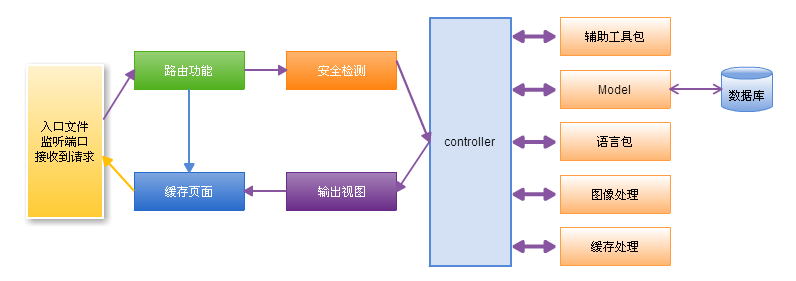
\includegraphics[width=14cm]{13.1.flow.png}
   \label{図13.3}
   \caption{フレームワークのデータフロー}
\end{figure}


\begin{enumerate}
  \item main.goはアプリケーションの入り口です。ブログを実行する上で必要となる基本的なリソースを初期化し、情報を設定し、ポートを監視します。
  \item ルーティング機能はHTTPリクエストを検査し、URLおよびmethodによって誰(コントローラ層)がリクエストのリソースへのリダイレクトを処理するかを決定します。
  \item もしキャッシュファイルが存在した場合、通常のプロセスを迂回して実行し、ブラウザに直接送信されます。
  \item セキュリティチェック:アプリケーションプログラムのコントローラがコールされる前にHTTPリクエストと任意のユーザが送信したデータがフィルタにかけられます。
  \item コントローラがモデル、コアライブラリ、補助関数および特定のリクエストに必要となるその他のリソースにおける任意の処理をロードします。コントローラは主に業務ロジックの処理に責任を負います。
  \item ビュー層において出力された内容はWebブラウザのコンテンツに送信されます。もしキャッシュが起動されていた場合、ビューはまずキャッシュされ、以降の通常のリクエストにおいて利用されます。
\end{enumerate}
